%% The following is a directive for TeXShop to indicate the main file
%%!TEX root = diss.tex
\chapter{Background and roadmap}
\label{ch:Introduction}

Optimization~\citep{bert:1999} refers to finding the minimum or maximum of a function given a set of constraints, which stays at the core of many fields, such as machine learning~\citep{sra2012optimization,Bubeck15}, data mining~\citep{shi2011optimization}, and signal processing~\citep{mattingley2010real,palomar2010convex}, to mention just a few. With big data and hardware technology development, optimization approaches are gaining increasing attention because of their broad applicability and attractive theoretical properties. In the meantime, in the fields such as computer vision~\citep{krizhevsky2012imagenet} and natural language processing~\citep{wolf2020transformers}, models might contain millions of variables, resulting in optimization problems with enormous dimensions. Because of this, computational efficiency is a significant problem that must be appropriately addressed, which necessitates the development of efficient and scalable optimization algorithms. 

In recent years, many significant breakthroughs have been made for computational efficiency regarding a class of optimization techniques known as the duality approach~\citep{combettes2011proximal,shalev2013stochastic,jaggi2014communication}. The main idea of the duality approach is to transform the original problem into a "dual" problem that has the same optimal value as the original problem under certain conditions and whose solution characterizes the optimality of the original problem. More importantly, it has been recognized that working on the dual of an optimization problem may significantly simplify its solution or enjoy a better convergence rate~\citep{komodakis2015playing}. 

\citet{rockafellar1970convex} developed a perturbation framework for studying the duality approach, which uses tools in convex analysis and the theory of conjugate function. This thesis investigates and extends the duality approach to two classes of optimization problems: structured optimization~\citep{bach2012optimization,chandrasekaran2012convex}, whose solution adopts some specific structural requirements, and federated learning~\citep{wang2021field}, which aims to learn models from decentralized data resources collaboratively. We also explore some exciting application scenarios of structured optimization in federated learning. 

For the rest of this chapter, \autoref{sec:1-1} introduces some basic notations and definitions that will be used in this thesis. We then review the duality perturbation framework in \autoref{sec:1-2}. Finally, in \autoref{sec:1-3} and \autoref{sec:1-4}, respectively, we introduce the backgrounds for structured optimization and federated learning, as well as the roadmap for the thesis. 

  

\section{Basic definitions and notations} \label{sec:1-1}

Unless otherwise specified, we use capital letters $A, B, \dots$ to denote matrices or linear operators, lowercase letters $a, b, \dots$ to denote vectors, calligraphic letters $\Ascr, \Bscr, \dots$ to denote sets, and Greek letters $\alpha, \beta, \dots$ to denote scalars.

We work with $n$-vectors in $\Real^n$ and $p$-by-$n$ matrices in $\Real^{p\times
n}$. The restriction to real-valued vectors and matrices considerably simplifies
our development, though many of the ideas set forth in this thesis extend to
more general functional spaces, as described by \citet{zalinescu2002convex} and
\citet{bauschke2011convex}.

Let $e_i$ denote the $i$th canonical unit vector, i.e., the vector of all zeros
except a single 1 in the $i$th position. The dot product of two $n$-vectors $x$
and $z$ is $\ip x z = \sum_{j} x_j z_j$. The dot product of two $p$-by-$n$
matrices $X$ and $Z$ is the trace inner product $\ip X Z = \trace(X\T Z) =
\sum_{ij}X_{ij}Z_{ij}$.

A vector norm $\|x\|$ always refers to the 2-norm, i.e., $\|x\| = \sqrt{\ip{x}{x}}$ unless otherwise specified. Matrix norms always refer to the Schatten norm, e.g., if $(s_1, s_2,\ldots)$ are
the singular values of $X$, then
\[
  \|X\|_1 = \sum_i s_i,
  \quad \|X\|_2=\Big(\sum_i s_i^2\Big)^{1/2},
  \text{and} \|X\|_\infty=\max_i s_i.
\]

The adjoint $M^*$ of any linear map $M$ is the unique
linear map that satisfies the relationship $\ip{Mx}{z}=\ip{x}{M^*z}$ for all $x$ and $z$. Thus, for
the linear map $M:\Real^n\to\Real^m$, the product of the adjoint and an
$m$-vector $y$ is $M^*y = \sum_{i=1}^m y_i (Me_i)$. For the linear map
$M:\Real^{p\times n}\to\Real^m$, the forward and adjoint maps take the form
\begin{equation} \label{eq:mat-map}
  M X = \begin{bmatrix}
    \ip{M_1}{X} \\ \vdots \\ \ip{M_m}{X}
  \end{bmatrix}  
  \quad\mbox{and}\quad
  M^*y = \sum_{i=1}^m y_i M_i,
\end{equation}
where each $M_i$ is a $p$-by-$n$ matrix. The notation $X\succeq0$
indicates that $X$ is symmetric positive definite.

A set $\Cscr$ is convex if
\[
    \forall (x, y, \lambda) \in \Cscr\times\Cscr\times[0,1], 
    \enspace \lambda x + (1-\lambda)y \in \Cscr. 
\]
A real-valued function $g:\Re^n\to\Re$ is convex if
\[
    \forall (x, y, \lambda) \in \Re^n\times\Re^n\times[0,1], 
    \enspace g\left(\lambda x + (1-\lambda)y\right) \leq \lambda g(x) + (1-\lambda)g(y). 
\]
Given a convex function $g:\Re^n\to\Re$ and a vector $x\in\Re^n$, the subdifferential of $g$ at $x$ is defined as 
\[\partial g(x) = \{z\in\Re^n \mid g(y) + \ip{z}{x - y} \leq g(x) ~\forall y \in \Re^n\}.\]
For any convex set $\Cscr$, its polar set is given by 
\begin{equation} \label{eq-polar-set}
    \Cscr\polar=\{z | \ip x z \le 1 \mbox{\ for all\ } x\in\Cscr \}.
\end{equation}
The indicator to $\Cscr$ is the
function
\[
  \delta\Cs(x) = \begin{cases}
    0 & \mbox{if $x\in\Cscr$;}
\\ +\infty & \mbox{otherwise}.
  \end{cases}
\]
The normal cone to $\Cscr$ at $x\in\Cscr$ is defined as
\[\Nscr\Cs(x) = \{d \mid \ip{d}{u - x} \leq 0 \mbox{ for all } u \in \Cscr\}.\]
The Euclidean projection onto $\Cscr$ is denoted
\[\proj\Cs(x) = \argmin{u \in \Cscr} \ \|x - u\|_2,\]
which defines the distance of a point to the set $\Cscr$, denoted by
\[\dist\Cs(x) = \|x - \proj\Cs(x)\|_2.\]

For any set $\Ascr$, its convex hull contains all
weighted averages of the elements of the set, denoted
\[
  \conv \Ascr =
  \left\{\sum_{i=1}^m \alpha_i x_i ~\bigg\vert~ x_i\in\Ascr,\ \alpha_i\ge0,\ \sum_{i=1}^m\alpha_i=1 \right\},
\]
for some some positive integer $m$. The conic extension of $\Ascr$ is defined by 
\[
  \cone\Ascr = \{\alpha d ~|~ d\in\Ascr,\ \alpha\ge0\}.
\]
The closure, boundary and relative interior, respectively,
of $\Ascr$ denoted $\cl\Ascr$, $\bnd\Ascr$ and $\ri\Ascr$. 
The gauge function with respect to $\Ascr$ is defined as the Minkowski functional to the closed convex hull of $\Ascr$, i.e.,
\begin{equation} \label{eq:gauge1}
    \gauge\As(x) = \inf\left\{\mu > 0 ~|~ x \in \mu\cl\conv(\Ascr\cup\{0\})\right\}.
\end{equation}
The support function with respect to $\Ascr$ is defined as 
\begin{equation} \label{eq:support}
    \sigma\As(z) = \sup\{\ip{a}{z} ~|~ a\in\Ascr\cup\{0\}\}.
\end{equation}
The descent cone of the set $\Ascr$ at point $x$ is defined as 
\[\Dscr(\Ascr, x) = \cone\{d\in \Re^n ~|~ \gauge\As(x + d) \leq \gauge\As(x)\}\]

Let $\Nscr(0,I)$ denote the standard Gaussian distribution. For a compact set $\Sscr$, $\uniform(\Sscr)$ denotes the uniform ditribution over $\Sscr$. For a convex cone $\Dscr$, let $\delta(\Dscr) \coloneqq \mE_{g\sim\Nscr(0,I)} \|\proj_{\Dscr}(g)\|_2^2 $ denote the statistical dimension of the cone $\Dscr$.

Consider a real-valued differentiable function $f:\Real^n\to\Real$. The function $f$ is $\alpha$-strongly convex for some $\alpha>0$ if $f$ satisfies
\[f(y) \geq f(x) + \ip{\nabla f(x)}{y-x} + \frac{\alpha}{2}\|x-y\|^2 \enspace \forall x, y \in \Re^n.\]
The function $f$ is $\beta$-smooth for some $\beta>0$ if $f$ satisfies
\[f(y) \leq f(x) + \ip{\nabla f(x)}{y-x} + \frac{\beta}{2}\|x-y\|^2 \enspace \forall x, y \in \Re^n.\]
The function $f$ is $\vartheta$-Lipschitz for some $\vartheta>0$ if $f$ satisfies
\[|f(x) - f(y)| \leq \vartheta\|x-y\| \enspace \forall x, y \in \Re^n.\]
The domain is denoted
$\dom f = \{x~|~f(x)<+\infty\}$, and the convex conjugate is denoted
\[
  f^*(z) = \sup_{x\in\Re^n}\{\ip x z - f(x) \}.
\] 

For any positive integer $N$, we use $[N]$ to denote the set $\{1, \dots, N\}$. 


\section{Duality in convex optimization} \label{sec:1-2}

Modern treatment of duality in convex optimization is based on an interpretation of multipliers as giving sensitivity information relative to perturbations in the problem data. The perturbation framework pioneered by \citet{rockafellar1970convex} plays an essential role in the duality theory. Here we briefly summarize this framework. 

Consider a general convex optimization problem
\begin{equation} \label{prob:general_cvx}
    \minimize{x \in \Re^n} f(x),
\end{equation}
where $f:\Re^n \to \Re$ is a closed convex function. The perturbation framework depends on an arbitrary convex perturbation function $F: \Re^n \times \Re^m \to \Re$ such that 
\begin{equation} \label{eq:value_fn_property}
    F(x, 0) = f(x) \enspace \forall x \in \Re^n.
\end{equation}
Then we define the corresponding value function $v_F : \Re^m \to \Re$ by
\begin{equation}
    v_F(u) = \inf_{x \in \Re^n} F(x, u).
\end{equation}
This set-up immediately yields the primal-dual pair
\begin{align}
    v_F(0) &= \inf_{x \in \Re^n} F(x, 0) \equiv f(x), \label{prob:general_primal}\\
    v_F^{**}(0) &= \sup_{y \in \Re^m} g(y) \coloneqq -F^*(0, y). \label{prob:general_dual}
\end{align}
By the property~\eqref{eq:value_fn_property} of the perturbation function $F$, we can see that problem~\eqref{prob:general_primal} is equivalent to the general convex optimization problem~\eqref{prob:general_cvx}. The problem~\eqref{prob:general_dual} is known as the \emph{dual} problem of~\eqref{prob:general_cvx} corresponding to the perturbation function $F$. 
The following theorem, developed by~\citet{rockafellar1998variational}, describes the relationship between the primal-dual pair:~\eqref{prob:general_primal} and~\eqref{prob:general_dual}. A simple geometric illustration is shown in~\autoref{fig:duality}.

\begin{figure}[t] 
    \begin{subfigure}{.48\textwidth}
      \centering
      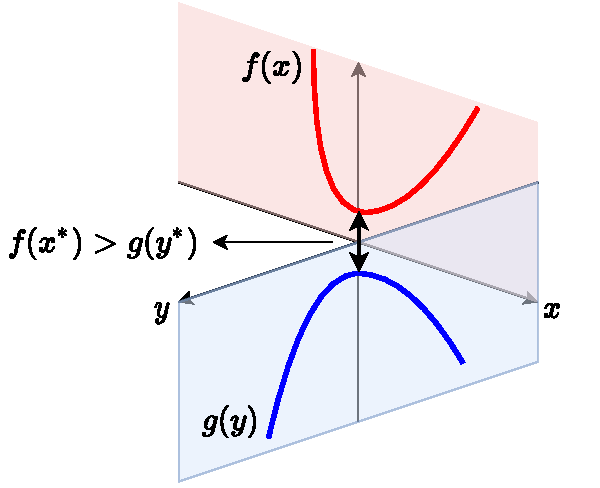
\includegraphics[width=\linewidth]{./figures/weak_dual.pdf}
      \captionsetup{justification=centering}
      \caption{Weak duality.}
    \end{subfigure}
    \hfill
    \begin{subfigure}{.48\textwidth}
      \centering
      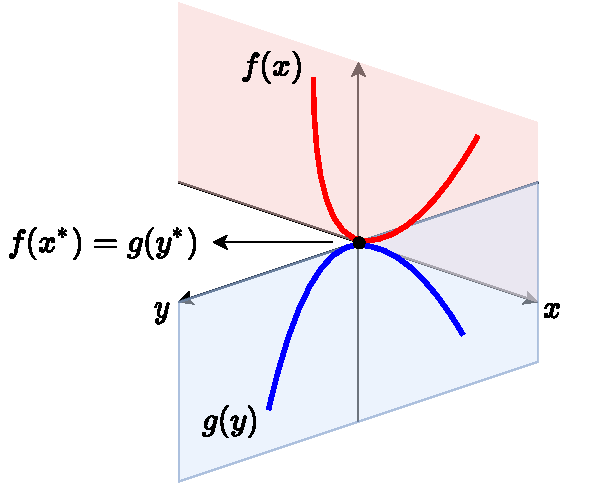
\includegraphics[width=\linewidth]{./figures/strong_dual.pdf}
      \captionsetup{justification=centering}
      \caption{Strong duality.}
    \end{subfigure}
    \captionsetup{justification=centering}
    \caption{Geometric illustration of weak and strong duality.}
    \label{fig:duality}
\end{figure}

\begin{theorem}[Duality theory~\protect{\citep[Theorem~11.39]{rockafellar1998variational}}] Consider the primal-dual pair:~\eqref{prob:general_primal} and~\eqref{prob:general_dual}, where $F: \Re^n \times \Re^m \to \Re$ is a proper, closed and convex function. The following properties hold. 
    \begin{itemize}
        \item \textbf{Weak duality}. The inequality $v_F(0) \geq v_F^{**}(0)$ always holds. 
        \item \textbf{Strong duality}. If $0 \in \ri\dom v_F \cup \ri\dom v_F^{**}$, then $v_F(0) = v_F^{**}(0)$. 
        \item \textbf{Optimal solutions.} If the strong duality holds with finite optimal values, then the following characterizations of the optimal solutions to the primal-dual pair are equivalent
            \begin{align}
                (x^*, 0) &\in \partial F^*(0,y^*); \\
                (0, y^*) &\in \partial F(x^*,0); \\
                v_F(0) = F^*(x^*, 0) &= -F^*(0,y^*) = v_F^{**}(0).
            \end{align}
    \end{itemize}
\end{theorem}

The perturbation function $F$ plays an important role in Fenchel-Rockafellar duality theory. Different choices of the perturbation function will lead to different dual problems. In the rest of this section, we will interpret three widely used primal-dual pairs: Lagrange dual, Fenchel dual and gauge dual, under this perturbation framework.  


\subsection{Lagrange duality}
Consider the general constrained convex optimization problem:
\begin{equation} \label{prob:general_constrained} 
    \minimize{x \in \Re^n} f(x) \st c_i(x) \leq 0 \enspace \forall i = 1, \dots, m,
\end{equation}
where $f:\Re^n\to\Re$ and $c_i:\Re^n\to\Re$ for all $i\in[m]$ are convex functions. In this case, the perturbation function is defined as 
\begin{equation}
    F(x, u) = f(x) + \sum_{i = 1}^m \delta_{\leq 0}(c_i(x) + u_i).
\end{equation}
Then we can derive the corresponding conjugate function as 
\begin{align*}
    -F^*(0, y) &= -\sup_{x\in\Re^n, u\in\Re^m} \ip{0}{x} + \ip{y}{u} - F(x,u)
             \\&= -\sup_{x\in\Re^n, w\in\Re_+^m} \sum_{i=1}^m \ip{y_i}{- c_i(x) - w_i} - f(x)
             \\&= 
             \begin{cases}
                 \inf_{x\in\Re^n} f(x) + \sum_{i=1}^m \ip{y_i}{c_i(x)} & \text{if} y \in\Re_+^m \\
                 -\infty & \text{otherwise}.
             \end{cases}
\end{align*}
Therefore, the Lagrange dual to problem~\eqref{prob:general_constrained} is given by
\begin{equation} \label{prob:general_constrained_dual}
    \maximize{y\in\Re_+^m} \minimize{x \in \Re^n} f(x) + \sum_{i=1}^m \ip{y_i}{c_i(x)}.
\end{equation}
The following theorem characterizes the duality for the Lagrange primal-dual pair. 

\begin{theorem}[Lagrange duality theory~\protect{\citep[Section~5.3]{boyd:2004}}] 
    Let $p^*$ and $d^*$ denote respectively the optimal values for the Lagrange primal-dual pair:~\eqref{prob:general_constrained} and~\eqref{prob:general_constrained_dual}. 
    \item \textbf{Weak duality}. $p^* \geq d^*$. 
    \item \textbf{Strong duality}. 
    If there exist an interior-point feasible point $\hat x$ for the primal problem~\eqref{prob:general_constrained}, i.e. $c_i(\hat x) < 0$ for $i = 1,\dots,m$, then $p^* = d^*$. Furthermore, let $x^*$ and $y^*$ denote respectively the optimal solutions to the primal-dual pair:~\eqref{prob:general_constrained} and~\eqref{prob:general_constrained_dual}, then 
    \[y_i^*c_i(x^*) = 0 \enspace \forall i = 1,\dots,m.\]
\end{theorem}


\subsection{Fenchel duality}
Consider the following optimization problem 
\begin{equation} \label{prob:general_fenchel} 
    \minimize{x \in \Re^n} f(x) + g(Mx),
\end{equation}
where $f:\Re^n\to\Re$ and $g:\Re^m\to\Re$ are closed convex functions, and $M:\Re^n\to\Re^m$ is a linear operator. In this case, the perturbation function is defined as 
\begin{equation}
    F(x, u) = f(x) + g(Mx + u).
\end{equation}
Then we can derive the corresponding conjugate function as
\begin{align*}
    -F^*(0, y) &= -\sup_{x\in\Re^n, u\in\Re^m} \ip{0}{x} + \ip{y}{u} - f(x) - g(Mx + u)
             \\&= -\sup_{x\in\Re^n} \left\{\sup_{u\in\Re^m} \ip{y}{Mx + u} - g(Mx + u)\right\} - f(x) - \ip{y}{Mx}
             \\&= - g^*(y) - \sup_{x\in\Re^n}\ip{-M^*y}{x} - f(x) 
             \\&= - g^*(y) - f(-M^*y).
\end{align*}
Therefore, the Fenchel dual to problem~\eqref{prob:general_fenchel} is given by
\begin{equation} \label{prob:general_fenchel_dual}
    \maximize{y\in\Re^m} - g^*(y) - f(-M^*y).
\end{equation}
The following theorem characterizes the duality for the Fenchel primal-dual pair. 

\begin{theorem}[Fenchel duality theory~\protect{\citep[Corollary 31.2.1]{rockafellar1970convex}}] 
    Let $p^*$ and $d^*$ denote respectively the optimal values for the Fenchel primal-dual pair:~\eqref{prob:general_fenchel} and~\eqref{prob:general_fenchel_dual}. 
    \item \textbf{Weak duality}. $p^* \geq d^*$. 
    \item \textbf{Strong duality}. 
    If $0\in\int(\dom g - M\dom f)$, then $p^* = d^*$. Furthermore, let $x^*$ and $y^*$ denote respectively the optimal solutions to the primal-dual pair:~\eqref{prob:general_fenchel} and~\eqref{prob:general_fenchel_dual}, then the following relationships hold
    \begin{align*}
          y^* &\in \partial g(Mx^*) \cap (M^*)^{-1}\partial f(x^*) \tand
        \\x^* &\in \partial f^*(-M^*y^*)\cap M^{-1}\partial g^*(y^*).
    \end{align*}
\end{theorem}




\subsection{Gauge duality}
Consider the following gauge optimization problem 
\begin{equation} \label{prob:general_gauge} 
    \minimize{x \in \Re^n} \gauge\Cs(x) \st Mx = b,
\end{equation}
where $\Cscr\subseteq\Re^n$ is a convex set and $\gauge\Cs$ is the corresponding gauge function, $M:\Re^n\to\Re^m$ is a linear operator, and $b\in\Re^m$ is a vector. By setting 
$\lambda \coloneqq 1/\gauge\Cs(x)$ and $w \coloneqq \lambda x$, problem~\eqref{prob:general_gauge} can be expressed as 
\begin{equation} \label{prob:general_gauge2} 
    \inf_{\lambda > 0, w \in \Re^n} \frac{1}{\lambda} \st w \in \Cscr \tand Mw = \lambda b.
\end{equation}
Note that minimizing $1/\lambda$ is equivalent to minimizing $-\lambda$ for $\lambda \geq 0$. In this case, the perturbation function is defined as 
\begin{equation}
    F(\lambda, w, u) = -\lambda + \delta\Cs(w) + \delta_{\{0\}}(\lambda b - Mw + u) + \delta_{\geq 0}(\lambda). 
\end{equation}
Then we can derive the corresponding conjugate function as
\begin{align*}
    -F^*(0, y) &= -\sup_{\lambda\in\Re, w\in\Re^n, u\in\Re^m} \ip{y}{u} + \lambda - \delta\Cs(w) - \delta_{\{0\}}(\lambda b - Mw + u) - \delta_{\geq 0}(\lambda)
    \\&= -\sup_{\lambda\in\Re, w\in\Re^n} \lambda - \delta\Cs(w) - \delta_{\geq 0}(\lambda) - \ip{\lambda b - Mw}{y}
    \\&= -\sup_{\lambda\geq 0} \delta\Cs^*(M^*y) + \lambda ( 1 - \ip{b}{y} )
    \\&= 
        \begin{cases}
            -\delta\Cs^*(M^*y) & \text{if} \ip{b}{y} \geq 1 \\
            -\infty & \text{otherwise}.
        \end{cases}
\end{align*}
Therefore, the gauge dual to problem~\eqref{prob:general_gauge} is given by
\begin{equation} \label{prob:general_gauge_dual}
    \maximize{y\in\Re^m} -\delta\Cs^*(M^*y) \st \ip{b}{y} \geq 1.
\end{equation}
The following theorem characterizes the duality for the gauge primal-dual pair. 

\begin{theorem}[Gauge duality theory~\protect{\citep[Theorem~5.1 and Corollary~5.2]{friedlander2014gauge}}] 
    Let $p^*$ and $d^*$ denote respectively the optimal values for the gauge primal-dual pair:~\eqref{prob:general_gauge} and~\eqref{prob:general_gauge_dual}. 
    \item \textbf{Weak duality}. If both primal problem~\eqref{prob:general_gauge} and dual problem~\eqref{prob:general_gauge_dual} are feasible, then $p^* d^* \geq 1$. 
    \item \textbf{Strong duality}. If either primal problem~\eqref{prob:general_gauge} or dual problem~\eqref{prob:general_gauge_dual} is strictly feasible and the other is feasible, then $p^* d^* = 1$. Furthermore, let $x^*$ and $y^*$ denote respectively the optimal solutions to the primal-dual pair:~\eqref{prob:general_gauge} and~\eqref{prob:general_gauge_dual}, then 
    \[\ip{x^*}{M^*y^*} = \gauge\Cs(x^*)\delta\Cs^*(M^*y^*).\]
    
\end{theorem}

\section{Structured optimization} \label{sec:1-3}

Convex optimization provides a valuable computational framework that renders many problems tractable because of the range of powerful algorithms that can be brought to the task. The key is that a specific mathematical structure, i.e., the convexity of the functions and sets defining the problem—opens an enormous range of theoretical and algorithmic tools that lend themselves astonishingly well to computation. However, there are limits to the scalability of general-purpose algorithms for convex optimization. As has been recognized in the optimization and related communities for at least the past decade, significant efficiencies can be gained by acknowledging the latent structure in the solution itself, coupled with the overarching structure provided by convexity.

Structured optimization proceeds by using a prescribed set of atoms to assemble an optimal solution. The atomic decomposition of a vector $x\in\Re^n$ with respect to an atomic set
$\Ascr\subset\Re^n$ is given by the weighted superposition
\begin{equation} \label{eq:atomic-decomp}
  x = \sum_{a\in\Ascr} c_a a, \quad c_a\ge0 \quad \forall a\in\Ascr.
\end{equation}
Each coefficient $c_a$ in the atomic decomposition measures the contribution of
the corresponding atom $a$ toward the representation of $x$. Intuitively, an
atomic decomposition reveals structural information implicit in a vector, with
large coefficients in the decomposition indicating the more significant
structures.

Within the context of an optimization problem, the atomic decomposition reveals
structural elements most significant in the minimization process.
In the simplest case, the atoms $\Ascr$ may be formed from the collection of
signed canonical unit vectors $\{\pm e_1,\ldots,\pm e_n\}$, which leads to the
atomic decomposition
\[
  x = \sum_{j=1}^n c_j a_j,
  \quad
  c_j: = |x_j|,
  \quad
  a_j:= (\sgn x_j)\cdot e_j.
\]
Trivially, the most significant atoms thus correspond to the variables $x_j$ in
the vector $x=(x_1,\ldots,x_n)$ with the largest magnitude.

This generic model for atomic decompositions was promoted by~\citet{cds98} in the context of sparse signal decomposition, and more recently, by~\citet{chandrasekaran2012convex}, who were concerned with obtaining sparse solutions to linear inverse problems. 

In this thesis, we want to answer the question of determining which of the atoms in the atomic set $\Ascr$ are essential to the atomic decomposition of $x$, and conversely, which atoms can be safely ignored. In \autoref{ch:Dual-Struc-Opt}, we study the atomic decomposition framework from a geometric perspective. Polarity, which extends the familiar notion of orthogonality from linear sets to general convex sets, plays a special role in a simple and geometric form of convex duality. This duality correspondence yields a general notion of alignment that leads to an intuitive and complete description of how atoms participate in the final decomposition of the solution. The resulting geometric perspective leads to variations of existing algorithms effective for large-scale problems. We illustrate these ideas with many examples, including applications in matrix completion and morphological component analysis. We further show that this dual alignment property allows us to design new structured optimization models for real-world applications and develop efficient and scalable algorithms for structured optimization problems. We briefly introduce the roadmap below. 

In \autoref{ch:App-Sig-Demix}, we study the signal demixing problem which seeks to separate a superposition of multiple signals into its constituent structural components. We propose a two-stage approach that first decompresses and subsequently deconvolves the noisy and undersampled observations of the superposition. Probabilistic error bounds are given on the accuracy with which this process approximates the individual signals. The theory of polar convolution of convex sets developed by~\citet{friedlander2019polarconvolution}, and the dual alignment property developed in \autoref{ch:Dual-Struc-Opt} play central roles in the analysis and solution process. If the measurements are random and the noise is bounded, this approach stably recovers low-complexity and mutually incoherent signals, with high probability and with optimal sample complexity. Numerical experiments on both real and synthetic data confirm the theory and the efficiency of the approach.

In \autoref{ch:App-Primal-Retrieval}, we study the structured data-fitting problem, which is prevalent in machine learning and data mining. In practice, people solve the corresponding structured convex relaxations. When tackling high-dimensional atomic-sparse optimization problems, dual-based algorithms are usually preferred over primal-based algorithms as dual variables usually live in a much lower-dimensional space than primal variables. One common issue of dual-based algorithms is that they still need to translate dual variables to primal variables at some point. How to retrieve a near-optimal primal variable efficiently with a provable guarantee is thus crucial for the success of dual approaches. We present a simple and computationally cheap strategy for retrieving a primal variable from any feasible dual variable based on the dual alignment property developed in \autoref{ch:Dual-Struc-Opt}. Theoretically, we show that our proposed strategy is capable of obtaining a near-optimal primal variable given a dual-based algorithm converging to the optimal dual solution. Numerical experiments on real-world datasets support our analysis.

In \autoref{ch:App-AtomicOpt}, we introduce our open-source package \texttt{AtomicOpt.jl} for solving a class of structured optimization problems, which is written in the Julia programming language~\citep{bezanson2017julia}. Our design depends on the level-set method~\citep{aravkin2016levelset}, a dual version of the conditional-gradient method~\cite{jaggi2013revisiting,frank1956algorithm,dunn1978conditional}, and the primal-retrieval strategy developed in~\autoref{ch:App-Primal-Retrieval}. The worst-case computational complexity of our algorithm is sublinear in the required accuracy. All the numerical experiments conducted in~\autoref{ch:Dual-Struc-Opt},~\autoref{ch:App-Sig-Demix} and~\autoref{ch:App-Primal-Retrieval} are reproducible via this package. 



 

\section{Federated learning} \label{sec:1-4}

With the development of artificial intelligence, people recognize that many powerful machine learning models are driven by large distributed datasets, e.g., AlphaGo~\citep{silver2016mastering} and AlexNet~\citep{krizhevsky2012imagenet}. In many industry-scale applications, training data is distributed in the form of silos, that is, training data is obtained and maintained by many data owners instead of being centralized at the place of a single owner or a data center. Because of industrial competition, privacy concerns, legal restrictions, and many other possible reasons, integrating or centralizing data from different sources faces enormous resistance and is often even infeasible~\cite{li2020review}. Federated learning, originally proposed by~\citet{federated2016}, is promising for training machine learning models on distributed data sources. It facilitates collaboration among a group of data owners (aka.~``clients'') and, at the same time, preserves their privacy. The central idea of federated learning is to periodically aggregate local models from clients to produce a more general and capable global model.

Federated learning can be further be classified into two main categories: horizontal federated learning and vertical federated learning~\cite{yang2019federated}. Horizontal federated learning refers to the scenarios where various clients' data sets share the same feature space but have separate sample IDs, and vertical federated learning refers to the scenarios where data sets owned by different clients share the identical sample IDs but have distinctive features. A simple characterization is shown in \autoref{fig:hfl_and_vfl}. 

\begin{figure}[t] 
    \begin{subfigure}{.48\textwidth}
      \centering
      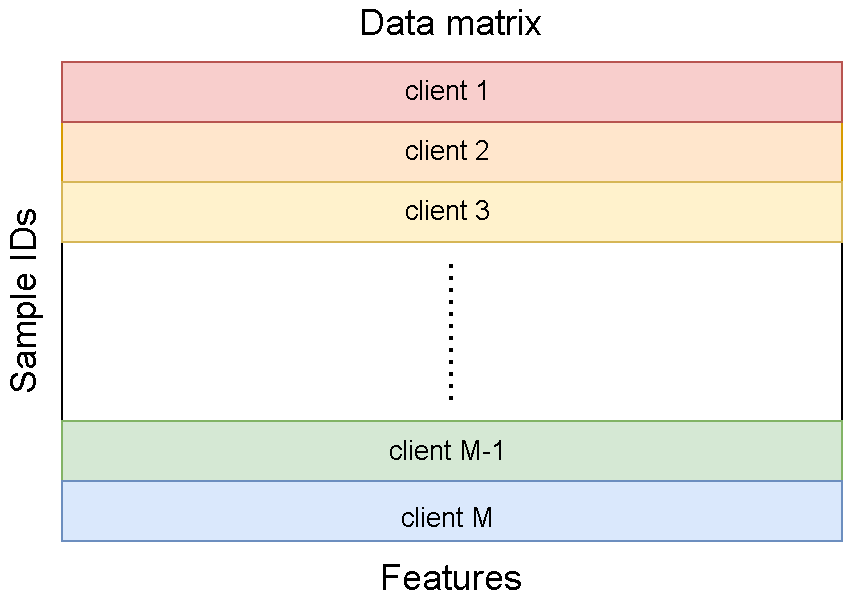
\includegraphics[width=\linewidth]{./figures/hfl_illustration.pdf}
      \captionsetup{justification=centering}
      \caption{Horizontal federated learning.}
      \label{fig:hfl}
    \end{subfigure}
    \hfill
    \begin{subfigure}{.48\textwidth}
      \centering
      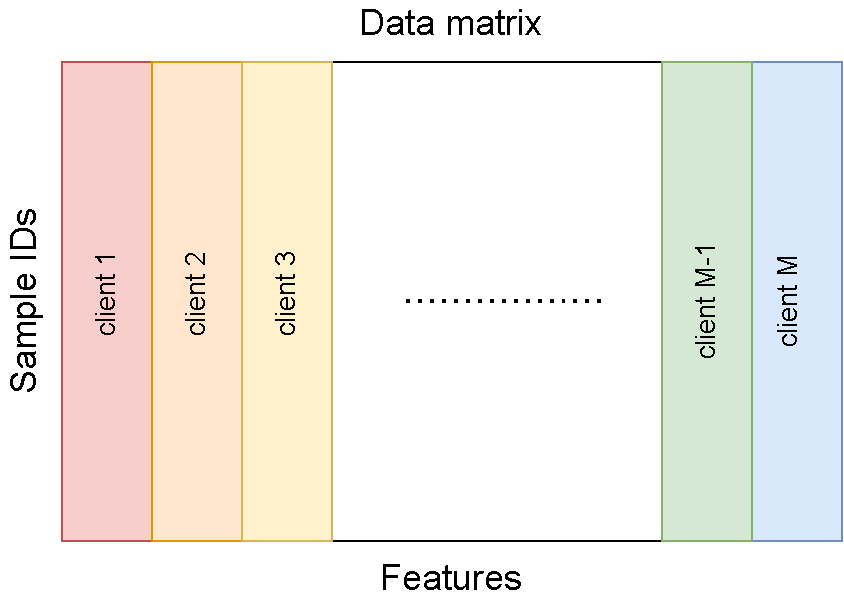
\includegraphics[width=\linewidth]{./figures/vfl_illustration.pdf}
      \captionsetup{justification=centering}
      \caption{Vertical federated learning.}
      \label{fig:vfl}
    \end{subfigure}
    \captionsetup{justification=centering}
    \caption{Characterization of horizontal and vertical federated learning.}
    \label{fig:hfl_and_vfl}
\end{figure}

This thesis shows that duality can be utilized to develop efficient and scalable algorithms for the optimization problem arising from federated learning. Besides, we show that structured optimization techniques can play an essential role in designing fair contribution valuation rules in federated learning. We briefly introduce the roadmap below. 

\subsection{Federated optimization} \label{sec:1-4-1}

A federated learning system is often composed of two components: clients and a central server at the physical level. The learning process in federated learning can be formulated as a distributed optimization problem, also known as federated optimization. As characterized and formalized by~\citet{wang2021field},~\citet{li2020federated} and~\citet{li2019convergence}, several essential characteristics distinguish FO from standard machine learning and distributed optimization. 

\begin{assumption}[Governing assumptions for federated optimization] \label{assum:govern}
The following assumptions hold for federated optimization. 
  \begin{itemize}
    \item \textbf{Slow Communication.}  Communication between clients and a central server is assumed to be the main bottleneck and dominates any computational work done at each of the clients. 
    \item \textbf{Data Privacy.} Clients want to keep their local data private, i.e., their data can not be accessed by any other client nor by the central server.
    \item \textbf{Data heterogeneity.} The training data are not independent and identically distributed (i.i.d.). In other words, a client’s local data cannot be regarded as samples drawn from single overall distribution.
    \item \textbf{Partial Participation.} Unlike traditional distributed learning systems, an FL system does not have control over individual client devices, and clients may have limited availability for connection. 
\end{itemize}
\end{assumption}

In \autoref{ch:Dual-Fed-Opt}, we study the federated optimization problem from a dual perspective. We propose a new algorithm termed federated dual coordinate descent (FedDCD), which is based on a type of coordinate descent method developed by \citet{necoara2017random}.  Additionally, we
enhance the FedDCD method with inexact gradient oracles and Nesterov's acceleration. We demonstrate
theoretically that our proposed approach achieves better convergence rates than the state-of-the-art
primal federated optimization algorithms under certain situations. Numerical experiments on real-world
datasets support our analysis.

\subsection{Contribution valuation in federated learning} \label{sec:1-4-2}

The effectiveness of federated learning depends on the active participation of motivated clients. Another important question in federated learning is how to ensure the clients’ long-term engagement, and how to motivate more clients' participation. One possible practical solution is to recompense the participated clients according to their contribution. 

Shapley value~\cite{shapley201617} is a classical measure originates from cooperative game theory to fairly assess contributions by participants in a coalition. 
The Shapley value of a participant is defined as the expectation of the marginal contribution of the participant over all possible subsets of the other participants. Shapley value is the unique measure that satisfies the four fundamental requirements of fairness proposed by Shapley~\cite{shapley201617}: balance, symmetry, zero element and additivity, which we formally define bellow. 

\begin{definition} \label{def:shapley}
    Supporse there are $M$ clientss and there is a black-box utility function $U:2^{[M]} \to \Re$ such that for any subset of clients $S \subseteq [M]$, the function $U(S)$ returns a utility score of the model collaboratively trained by the clients in $S$, such as the performance of the model. Let $v: [M] \to \mathbb{R}$ be the evaluation metric associated with the utility function $U$. The metric $v$ is called \emph{Shapley-fair} with respect to $U$ if it satisfies the following for fundamental requirements
    \begin{enumerate}
        \item \textbf{Symmetry.} For any two clients $i, j \in [M]$, if for any subset of clients $S \subseteq [M] \setminus \{i,j\}$, $U(S \cup \{i\}) = U(S \cup \{j\})$, then $v(i) = v(j)$. 
        \item \textbf{Zero element.} For any client $i \in [N]$, if for any subset of clients $S \subseteq [M] \setminus \{i\}$, $U(S \cup \{i\}) = U(S)$, then $v(i) = 0$.
        \item \textbf{Additivity.} If the utility function $U$ can be expressed as the sum of separate utility functions, namely $U = U_1 + U_2$ for some $U_1, U_2 : 2^I \to \mathbb{R}$, then for any client $i \in [M]$, $v(i) = v_1(i) + v_2(i)$, where $v_i$ and $v_2$ are the evaluation metrics associated with the utility functions $U_1$ and $U_2$, respectively. 
        \item \textbf{Balance.}  $U([M]) = \sum_{i \in [M]} v(i)$.
    \end{enumerate}
\end{definition}

Under the federated learning setting, a utility function is usually defined using the model performance on a data set. The symmetry requires that the same contributions to the utility should receive the same evaluation, which implies that clients with same local data sets should receive same evaluation. The zero element requires that no contribution, no value is recognized. The additivity requires that if there are multiple tasks and thus multiple test data sets, then the contributions of any client with respect to the test data sets can be expressed as the sum of the contributions with respect to those different tasks and test data sets. Note that, although balance is a necessary condition in many economic contests because it ensures payment is fully distributed to all clients, it is irrelevant in the context of our paper because we are only concerned about the relative contributions of clients. It is shown~\cite{dubey1975uniqueness,ghorbani2019data} that if the data valuation metric $v$ satisfies symmetry, zero element, and additivity, then $v$ must have the form
\begin{equation} \label{eq:shapley}
    v(i) = c \sum\limits_{S \subseteq I \setminus\{i\}} \frac{1}{\binom{N-1}{|S|}} \left[U(S\cup\{i\}) - U(S)\right],
\end{equation}
for some positive constant $c$.  

Although Shapley value has many desirable properties, evaluating Shapley value in federated learning requires exhaustive retraining and evaluating the model on every subset of clients. The costs of communication and time may be prohibitive in practice~\cite{song2019profit}. To tackle this challenge, some variations inspired by Shapley value were developed. Federated Shapley value (FedSV), recently proposed by \citet{wang2020principled}, is a measure for valuating contribution under the framework of horizontal federated learning. The key idea is to compute the Shapley values for clients in each round of training and then report the summation over all the rounds as the final results. This design cleverly avoids model retraining. However, there are still factors of potential unfairness in the design of FedSV because two data owners with the same local data may not receive the same evaluation. 

In \autoref{ch:Val-HFL}, we propose a new measure called completed federated Shapley value (ComFedSV) for contribution valuation in horizontal federated learning, which improves the fairness of FedSV. The design depends on completing a matrix consisting of all the possible contributions by different subsets of the data owners. It is shown under mild conditions that this matrix is approximately low-rank by leveraging concepts and tools from structured optimization. Both theoretical analysis and empirical evaluation verify that the proposed measure does improve fairness in many circumstances.

In \autoref{ch:Val-VFL}, we extend the idea of FedSV to vertical federated learning. We propose a contribution valuation metric called vertical federated Shapley value (VerFedSV), which utilizes tools from structured optimization. We show that VerFedSV not only satisfies many desirable properties for fairness but is also efficient to compute, and can be adapted to both synchronous and asynchronous vertical federated learning algorithms. Both theoretical analysis and extensive experimental results verify the fairness, efficiency, and adaptability of VerFedSV.




